\chapter{Описание практической части}
\label{sec:Chapter4} \index{Chapter4}

\section{Реализация предложенных улучшений}

В этом разделе описана реализация алгоритма пропагации инвариантов цикла в тело цикла с учетом предложенных улучшений в компиляторной инфраструктуре LLVM.

\subsection{Обработка циклов функции}

Циклы внутри функции обходятся в следующем порядке: все вложенные циклы обрабатываются перед обработкой внешнего цикла.

Для каждого цикла строится множество \enquote{холодных} блоков -- базовых блоков, доминируемых предзаголовком и имеющих оценку частоты исполнения меньше, чем у предзаголовка.
Это множество представлено в коде программы как две структуры: сортированный по возрастанию частоты базового блока массив указателей на блоки и хеш-таблицы нумерации \enquote{холодных} блоков, которая предоставляет соответствие между значением указателя и индексом в массиве.
Хеш-таблица используется впоследствии для обеспечения определенности порядка исполнения программы.

После чего алгоритм переходит к обработке инструкций предзаголовка цикла.

\subsection{Обработка инструкций предзаголовка цикла}

Инструкции предзаголовка обходятся в обратном порядке.
Это упрощает сохранение зависимостей между инвариантами.
Пусть существуют два инварианта $a$ и $b$.
$b$ использует значение $a$, а следовательно, $b$ расположен ближе к началу предзаголовка, чем $a$.
Тогда если инвариант $a$ будет спропагирован раньше, чем $b$, цепь определение-использование будет нарушена в ходе трансформации, и обеспечения корректности потребует дополнительных операций.
Для каждой инструкции, не имеющей стороних эффектов:
\begin{itemize}
    \item Строится множество базовых блоков, содержащих использование инструкции, или, в случае если инструкция используется в $\varphi$-узле, блоков, из которого поток управления приходит в $\varphi$-узел с значением инварианта.
    \item Затем строится множество базовых блоков, в которые будет производиться пропагация $M$.
        \begin{itemize}
            \item $M$ инициализируется как копия множества блоков использований инварианта.
            \item Для каждого блока из множества \enquote{холодных} базовых блоков:
                \begin{itemize}
                    \item Строится множество блоков из $M$, которые доминируются \enquote{холодным} блоком.
                    \item Если суммарная частота базовых блоков этого множества больше, чем частота \enquote{холодного} блока, блоки заменяются в множестве $M$ на \enquote{холодный} блок.
                \end{itemize}
        \end{itemize}
    \item Если суммарная частота блоков множества $M$ больше частоты предзаголовка, инвариант не пропагируется.
    \item Если в $M$ единственный блок, инвариант пропагируется в этот блок.
    \item Иначе, указатели на базовые блоки из множества $M$ копируются в массив.
        Этот массив сортируется по возрастанию значений хеш-таблицы нумерации \enquote{холодных} блоков.
    \item В каждый блок из полученного массива вставляется копия инструкции, порождающей инвариант, и все использования оригинальной инструкции в доминируемых блоках заменяются на использование копии, оригинальная инструкция удаляется.
\end{itemize}

\section{Анализ асимптотики алгоритма}

В этом разделе рассчитывается асимптотика описанного алгоритма.

\subsection{Асимптотика времени построения множества $M$}
Построение множества $M$ имеет асимптотику $ O(|U| |C|) $, где $C$ -- множество \enquote{холодных} базовых блоков, $U$ -- множество базовых блоков, содержащих использование инварианта.
Оба этих числа могут иметь порядок числа блоков цикла.
Поэтому, для ограничения времени исполнения трансформации линейной функцией от числа блоков цикла, вводится дополнительный параметр $|U|_{max}$.
Если $|U|$ превышает значение этого параметра, такой инвариант не рассматривается.
Это не оказывает сильного влияние на эффективность алгоритма, так как для инварианта с большим числом использований маловероятно найти множество $M$, удовлетворяющее поставленным требованиям.

\subsection{Асимптотика времени пропагации инварианта}

Копирование инструкции в блоки множества $M$ и замена использований инструкции занимает:
\begin{equation} \label{eq:copy_assimp}
    O(|M| N_u)
\end{equation}
Где $N_u$ - число использований инструкции.

По построению множества $M$:
$$ |M| \leq |U| $$
При этом $|U|$ ограничен сверху константой $|U|_{max}$.

Строго говоря, число использований может нелинейно зависеть от числа блоков, содержащих использования $|U|$.
Однако, его можно ограничить сверху произведением общего числа инструкций в блоках множества $U$ на константу $C$ -- максимальным числом аргументов инструкции:

\begin{equation} \label{eq:sum_leq_one}
N_u \leq C \; \sum_{b \in U} N_b
\end{equation}

Тогда выражение \ref{eq:copy_assimp} приводится к виду:

$$ O(|U|_{max} \; C \sum_{b \in U} N_b) = O(\sum_{b \in U} N_b) $$

\subsection{Асимптотика времени работы над циклом}

Из рассуждений выше, следует, что асимптотика времени исполнения алгоритма над некоторым циклом будет равна:
\begin{equation} \label{eq:loop_assimp}
O(N_p \; \sum_{i \in P} {\sum_{b \in U_i} N_b})
\end{equation}
Где:
\begin{itemize}
    \item $N_p$ -- число инструкций предзаголовка.
    \item $P$ -- множество инструкций предзаголовка.
    \item $U_i$ -- множество блоков, содержащих использование инварианта $i$.
\end{itemize}

Аналогично \ref{eq:sum_leq_one}:
$$ \sum_{i \in P} {\sum_{b \in U_i} N_b} \leq C \; N $$
Где $N$ -- число инструкций в функции.

Тогда \ref{eq:loop_assimp} приводится к виду:

$$ O(N_p \; N) $$

\subsection{Асимптотика времени обработки функции}

Асимптотика времени обработки функции имеет вид:
\begin{equation} \label{eq:assimp}
O(N \sum_{l \in L} N_{p_l})
\end{equation}
Где $L$ -- множество циклов функции, $N_{p_l}$ -- число инструкций в предзаголовке цикла $l$.

Каждый цикл обладает уникальным предзаголовком, а следовательно:
$$ \sum_{l \in L} N_{p_l} \leq N $$
Таким образом, в худшем случае, асимптотика алгоритма имеет вид:
\begin{equation} \label{eq:assimp_worst}
O(N^2)
\end{equation}

В среднем, число циклов и инструкций в предзаголовке цикла много меньше числа общего числа инструкций функции.
$$ |L| << N, N_{p_l} << N $$

Исходя из этого утверждения, средняя асимптотика времени работы алгоритма:
\begin{equation} \label{eq:assimp_worst}
O(N)
\end{equation}

\section{Анализ производительности}

Для анализа производительности произведенных изменений были измерены изменения числа исполненых инструкций на наборе бенчмарков SPEC CPU\textsuperscript{\tiny\textregistered} 2017 и наборе бенчмарков из коллекции тестов LLVM.

\subsection{Методика измерений}

Измерения проводились на системе на кристале Alibaba T-Head XuanTie C910 ICE под управлением операционной системы Линукс.
Процессор этой системы имеет 2 ядра.
Все бенчмарки запускались в однопоточном режиме, второе ядро системы не нагружалось.
Тактовая частота процессора была зафиксирована и составляла 1.2 ГГц.
Процессор имеет архитектуру набора команд RISC-V 64 GC.

Измерялись время исполнения программы в тактах и число исполненных инструкций.
Сравнение времени исполнения программы позволяет оценить влияние улучшения на общую производительность целевой платформы.
Сравнение числа исполненных инструкций позволяет выделить влияние платформонезависимой оптимизации, так как не учитывает среднее время исполнения инструкции, которое в большей мере зависит от микроархитектуры процессора, чем от исполняемого кода.

Для сбора метрик использовалась программа perf.
Эта программа позволяет собирать значения соответствующих счетчиков процессора, тем самым обеспечивая наиболее точные значения собираемых метрик при непосредственном исполнении на целевой машине.

Анализ производительности трансформации проводился с использованием динамического профилирования.
Как было показано в главе \ref{sec:Chapter2}, это позволяет получить наиболее точную информацию о частоте исполнения базовых блоков, и тем самым, оценить производительность алгоритма расположения инвариантов отдельно от точности анализа вероятности переходов.

Измерения производились следующим образом:
\begin{itemize}
    \item Код программы компилировался с включенной инструментацией кода для генерации динамического профиля.
    \item Полученный исполняемый файл запускался для сбора профиля исполнения программы.
    \item Код программы компилировался повторно, с использованием собранного профиля.
    \item Полученный исполняемый файл запускался под управлением программы perf для сбора метрик.
\end{itemize}

\subsection{SPEC CPU\textsuperscript{\tiny\textregistered} 2017}

Результат вышеописанных измерений для набора бенчмарков SPEC CPU\textsuperscript{\tiny\textregistered} 2017 представлен на графиках \ref{fig:plot_spec_both}.

\begin{figure}
    \centering
    \begin{subfigure}{0.4\textwidth}
        \centering
        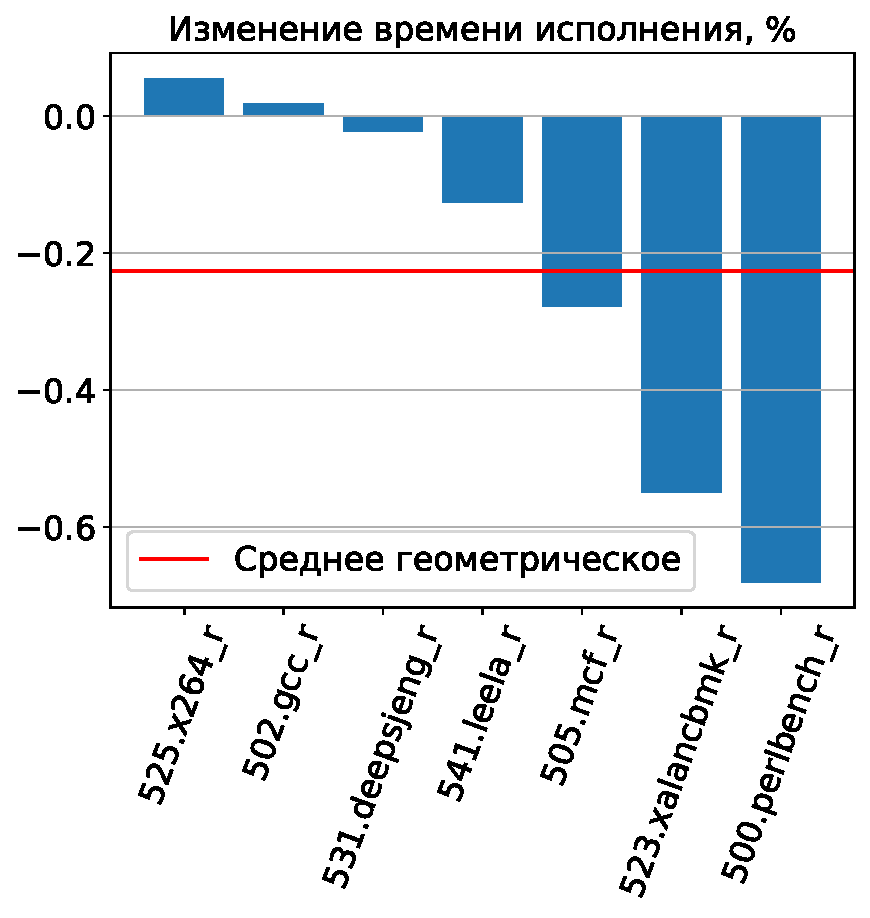
\includegraphics[width=\linewidth]{plot_spec_both_cycles.pdf}
    \end{subfigure}
    \begin{subfigure}{0.4\textwidth}
        \centering
        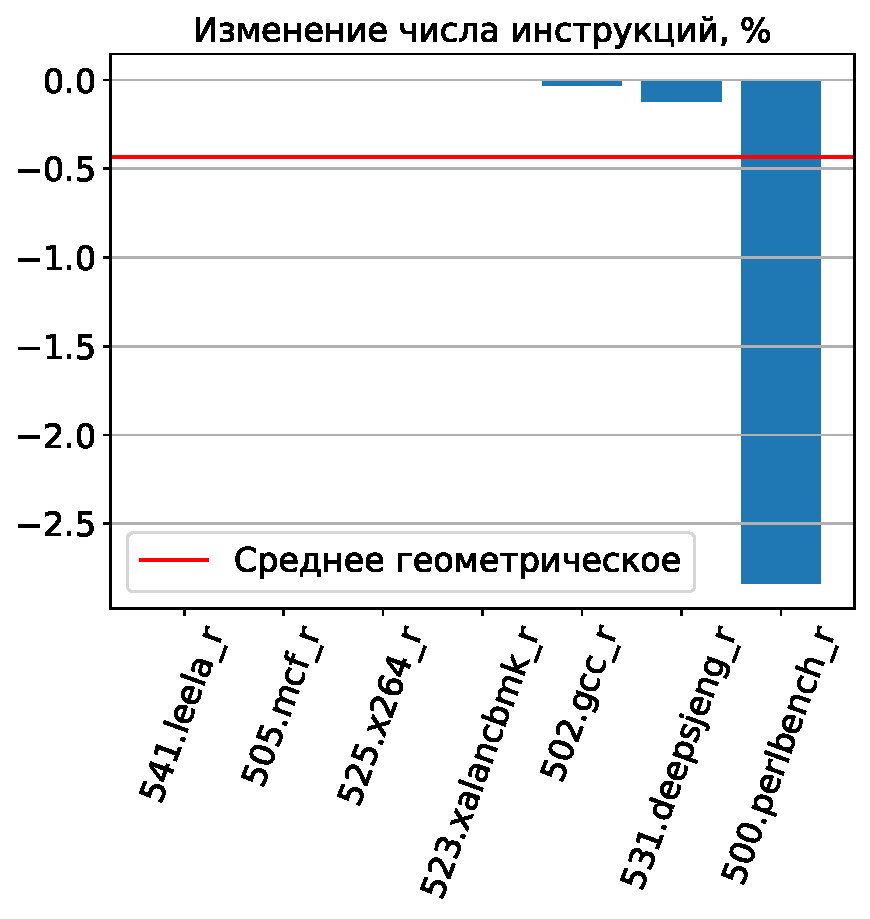
\includegraphics[width=\linewidth]{plot_spec_both_instructions.pdf}
    \end{subfigure}
    \caption{Сравнение производительности на SPEC CPU\textsuperscript{\tiny\textregistered} 2017}
    \label{fig:plot_spec_both}
\end{figure}

На графике видно уменьшение по обеим метрикам, особенно на бенчмарке \enquote{500.perlbench\_r}, что свидетельствует об эффективности произведенных улучшений.

\subsection{Коллекция тестов LLVM}

Бенчмарки из этого набора имеют значительно меньший размер, поэтому, для уменьшения погрешности, вносимой операционной системой, собиралось среднее значение метрик по результатам нескольких последовательных запусков набора бенчмарков.
Результат измерений представлен на графиках \ref{fig:plot_micro_both}.
На графиках программы набора отсортированы по убыванию значения метрики.

Можно видеть, что в большинстве случаев, метрики убывают.
Рост числа инструкций на некоторых тестах связан с неточностью профиля и погрешностью измерений.
Среднее геометрическое изменений значений метрики меньше нуля для каждой метрики, что свидетельствует об улучшении производительности.

\begin{figure}
    \centering
    \begin{subfigure}{0.4\textwidth}
        \centering
        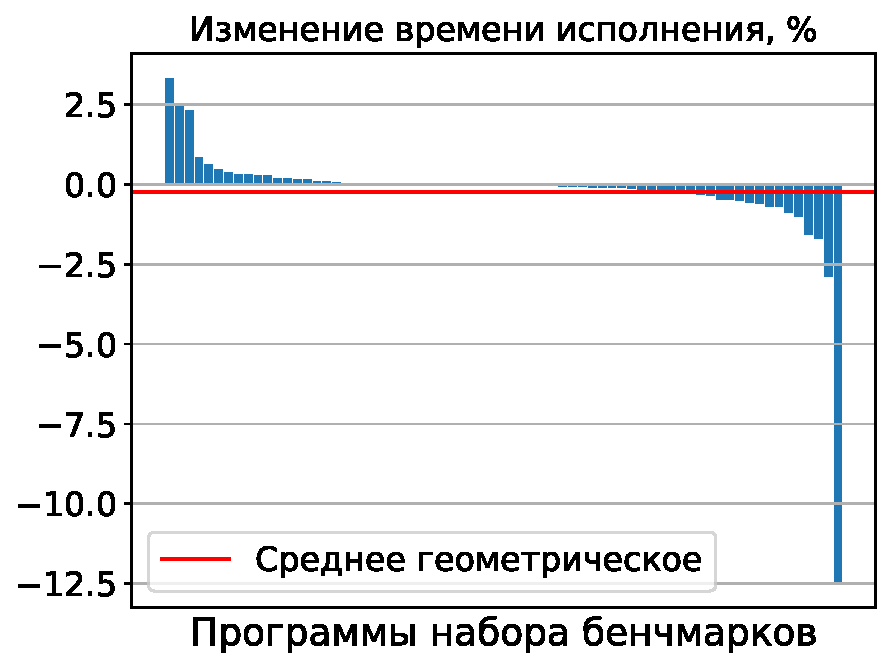
\includegraphics[width=\linewidth]{plot_micro_both_cycles.pdf}
    \end{subfigure}
    \begin{subfigure}{0.4\textwidth}
        \centering
        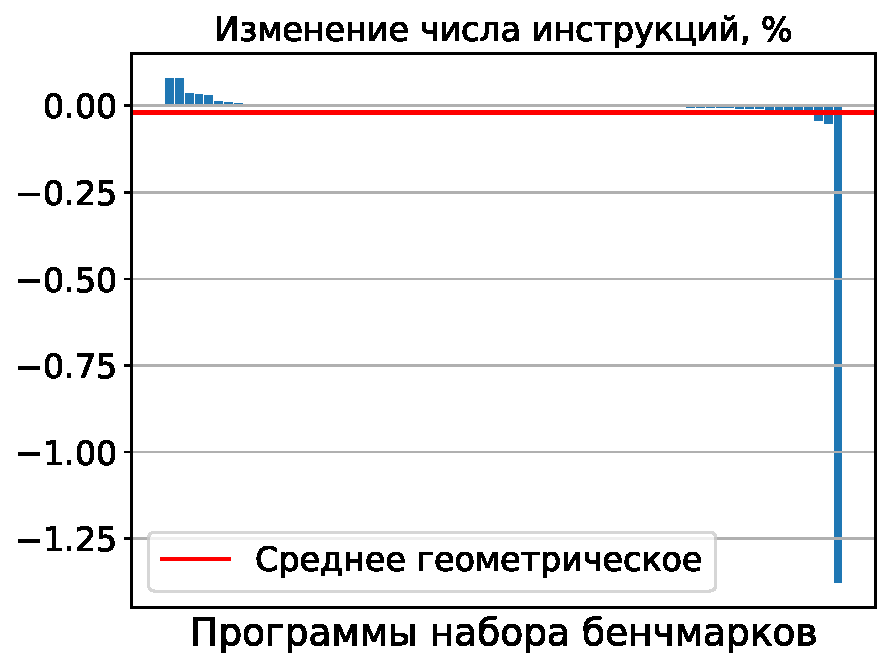
\includegraphics[width=\linewidth]{plot_micro_both_instructions.pdf}
    \end{subfigure}
    \caption{Сравнение производительности на наборе из коллекции тестов LLVM}
    \label{fig:plot_micro_both}
\end{figure}

\newpage
